\section{Techniques for Evaluating Limits}


To start, then, two easy limits.

\subsection*{Two Easy Limits}
\begin{enumerate}
  \item Let $f(x) = k$, where $k$ is some real number.
  Then $\dlim_{x\to a} k = k$.

  \begin{describe}{\textit{Explanation}}
    This function is a constant function, meaning that every output of the function is $k$, no matter what the input is.\\

    That means that for every $x$, $f(x) = k$. So then for all $x$ that are close to $a$, $f(x) = k$.\\

    So $f(x)$ is arbitrarily close to $k$ (in fact, it's equal to $k$) for all $x$ sufficiently close to, but not equal to, $a$.\\

    Visually, we can see some graphical evidence of this.
    \begin{figure}[h!tb]
      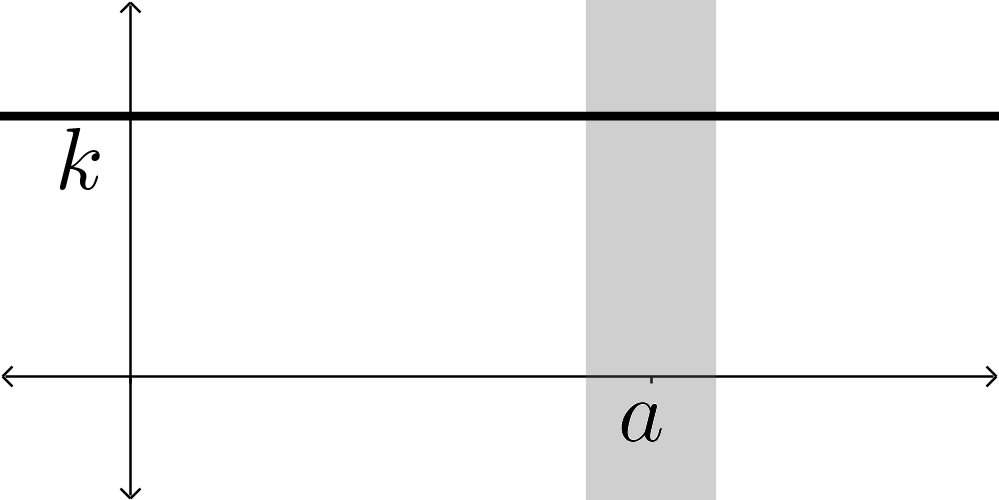
\includegraphics[scale=0.5]{./1_limits/images/1-2_graph1.png}
      \centering
    \end{figure}
  \end{describe}
  \item Let $f(x) = x$. Then $\dlim_{x\to a} x = a$.

  \begin{describe}{\textit{Explanation}}
    This function is the identity function, meaning that every output of the function is the same as the input.\\

    Then, when $x$ is close to $a$, $f(x) = x$ is also close to $a$.
    In fact, $f(x)$ is as close to $a$ as $x$ is, since they're the same thing.
    Thus, $f(x)$ is arbitrarily close to $a$ whenever $x$ is sufficiently close to $a$.\\

    Visually, we can see some graphical evidence of this.
    \begin{figure}[h!tb]
      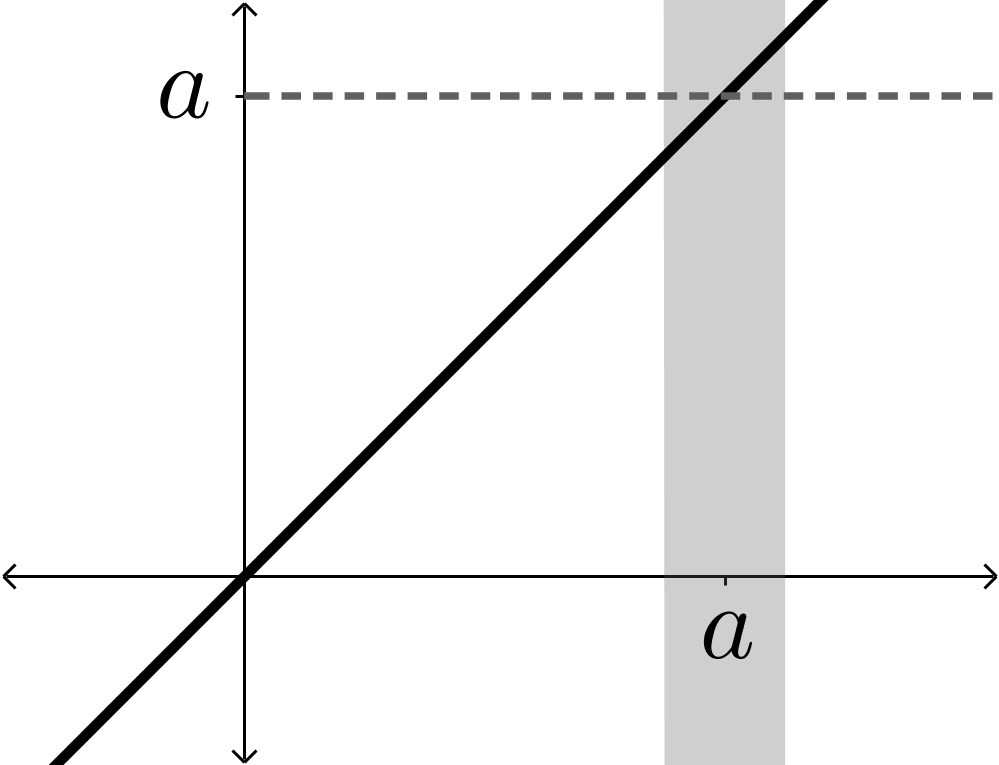
\includegraphics[scale=0.5]{./1_limits/images/1-2_graph2.png}
      \centering
    \end{figure}
  \end{describe}
\end{enumerate}

\begin{note}{Examples}
  There really isn't much to do here, since once you've seen a couple of these examples, you've essentially seen them all.

  \begin{enumerate}
    \item $\dlim_{x\to 4} -3 = -3$
    \item $\dlim_{x\to -8} 7 = 7$
    \item $\dlim_{x\to -1} x = -1$
    \item $\dlim_{x\to 15} x = 15$
  \end{enumerate}
\end{note}

\begin{note}{Examples}
  Notice that polynomials and rational functions become kind of easy:
  \begin{enumerate}
    \item $\dlim_{x\to 4}x^3-5x^2+3x-4$
    \item $\dlim_{x\to -2} \dfrac{x^2+1}{x^2-5x-1}$
  \end{enumerate}
\end{note}

Essentially, we're able to just plug values in for any polynomial function or rational function.
When might this screw up for rational functions?

\begin{thm}{Limits of Polynomial and Rational Functions}
  Let $p$ and $q$ be polynomials and let $a$ be some constant.
  Then:
  \begin{itemize}
    \item $\dlim_{x\to a} p(x) = p(a)$
    \item $\dlim_{x\to a} \dfrac{p(x)}{q(x)} = \dfrac{p(a)}{q(a)}$ as long as $q(a)\neq 0$
  \end{itemize}
\end{thm}

So, what happens when $\dlim_{x\to a} f(x) \neq f(a)$?
What if we have a rational function that does not exist at a certain point?

\begin{note}{Remember}
  The limit of $f(x)$ as $x\to a$ does not depend on the actual function value at $x=a$.
\end{note}

\begin{note}{Examples}
  \begin{multicols}{2}
    \begin{enumerate}
      \item $\dlim_{x\to2} \dfrac{x^2-6x+8}{x^2-4}$
      \item $\dlim_{x\to1} \dfrac{\sqrt{x}-1}{x-1}$
    \end{enumerate}
  \end{multicols}
\end{note}

\subsection*{Reality Check}

We've got some tools to evaluate limits analytically, and that's great.
We probably feel pretty good.
Limits aren't so bad!
But there are still some important limits that we'll struggle with analytically.

\begin{note}{Example}
  Estimate the slope of the line tangent to $f(x) = 2^x$ at point $(0,1)$.

  Just like we did to start the semester, we'll need to set up the slope of a secant line between some point $(x, 2^x)$ and our point $(0,1)$.
  Then we can take a limit as $x\to0$: $\dlim_{x\to0} \dfrac{2^x-1}{x}$.

  Technically we need to check both sides of the limit, but let's just check one side numerically.
   Set up a chart with values for $x$.
\end{note}

\section*{The Squeeze Theorem}

This will be another tool for calculating tricky limits.
Essentially what we'll do is try to trap (or squeeze) our function in between two other functions that have the same limit as $x\to a$.
Then we'll know the limit of our function as $x \to a$.

\begin{thm}{The Squeeze Theorem}
  Assume fucntions $f$, $g$, and $h$ satisfy $f(x) \leq g(x) \leq h(x)$ for all values of $x$ near $a$ (except possibly at $a$ itself).
  If $\dlim_{x\to a} f(x) = \dlim_{x\to a} h(x) = L$, then $\dlim_{x\to a} g(x) = L$ also.
\end{thm}

\begin{itemize}
  \item Squeeze $g(x) = \sin x$ between $f(x) =-|x|$ and $g(x) = |x|$ for $x\to 0$.
  \item Squeeze $g(x) = \cos x$ between $f(x) =1$ and $g(x) = |x|+1$ for $x\to 0$.
  \begin{note}{Note}
    Shift everything down 1 unit if it's easier.
  \end{note}
\end{itemize}

\begin{note}{Example}
  Use the Squeeze Theorem to find the limit $\dlim_{x\to 0} x^2\sin(1/x)$.

  The first problem is to think about which functions to use.
  This isn't always easy.
  We need a function that is greater than $x^2\sin(1/x)$ around $x=0$ and a function that is less than $x^2\sin(1/x)$ around $x=0$.

  \textbf{\textit{Notice:}}
  We can put some inequalities around trig functions that might help.
  For any angle $\theta$, we know that $-1\leq \sin \theta \leq 1$.
  So if the angle $\theta = 1/x$, then we know that $-1\leq \sin(1/x) \leq 1$.

  So $-x^2 \leq x^2 \sin (1/x) \leq x^2$.
  This makes things REALLY easy!
  \[-x^2 \leq x^2 \sin (1/x) \leq x^2 \to \dlim_{x\to0} -x^2 \leq \dlim_{x\to0} x^2 \sin (1/x) \leq \dlim_{x\to0} x^2\]

  But we know that $\dlim_{x\to0} -x^2 = \dlim_{x\to0} x^2 = 0$.
  So $0\leq \dlim_{x\to0} x^2 \sin (1/x) \leq 0$ which tells us that $\dlim_{x\to0} x^2 \sin (1/x)=0$.
\end{note}
